%-------------------------------------------------------------------------------------- Início
\begin{frame}[fragile,t]{Ruby} 
  \begin{itemize}
    \item Linguagem inventada por Yukihiro \alert{"Matz"} Matsumoto
    \item Versão \alert{1.0} liberada em \alert{1996}(Japão)
    \item \alert{Popularizada} no início de 2005 pelo \alert{Rails}
  \end{itemize}   
  \begin{figure}[hbt]
    
\includegraphics[scale=.5]{imagens/matz.jpg}
  \end{figure}
\end{frame}
%-------------------------------------------------------------------------------------- Início
\begin{frame}[fragile,t]{Ruby}
  \begin{itemize}
    \item Linguagem \alert{dinâmica} e \alert{orientada a objetos}
    \item Elegante, \alert{expressiva} e declarativa
    \item Influenciada pelo Perl, Smalltalk, Eiffel e Lisp
  \end{itemize}   
\end{frame}
%-------------------------------------------------------------------------------------- Início
\begin{frame}[fragile,t]{..Java..}
  \begin{lstlisting}[style=JavaInputStyle]
    public class Print3Times {
      public static void main(String[] args) {
        for(int i = 0; i < 3; i++) {
          System.out.println("Hello World!")
        }
      }
    }
  \end{lstlisting}
\end{frame}
%-------------------------------------------------------------------------------------- Início
\begin{frame}[fragile,t]{..Ruby..}
		\lstinputlisting[style=RubyInputStyle, caption=hello.rb]{codigos/ruby/01-ruby-introducao/hello.rb}
\end{frame}
%-------------------------------------------------------------------------------------- Início
\begin{frame}[fragile,t]{Básico do Ruby}
  \begin{itemize}
    \item Indentação de \alert{2 espaços} para cada nível aninhado (\alert{recomendado})
    \item \# é utilizado para comentários
    \begin{itemize}
    	\item use com moderação, o código deve ser \alert{auto documentado}
    \end{itemize}
    \item Scripts utilizam a extensão \verb!.rb! 
		\lstinputlisting[style=RubyInputStyle, caption=hello.rb]{codigos/ruby/01-ruby-introducao/hello.rb}
  \end{itemize}   
\end{frame}
%-------------------------------------------------------------------------------------- Início
\begin{frame}[fragile,t]{Saída na Tela}
  \begin{itemize}
    \item \verb!puts! é método \alert{padrão} para impressão em tela 
    \begin{itemize}
    	\item insere uma quebra de linha após a impressão
    	\item similar ao \verb!System.out.println! do Java
    \end{itemize}
    \item \alert{p} é utilizado para depuração
  \end{itemize}   
\end{frame}
%-------------------------------------------------------------------------------------- Início
\begin{frame}[fragile,t]{Entrada pelo Teclado}
  \begin{itemize}
    \item \verb!gets! é método \alert{padrão para receber} um valor pelo teclado 
		\begin{lstlisting}[style=RubyInputStyle]
# recebe um valor do tipo string.
nome = gets
  	\end{lstlisting}
    \item Utilize \verb!gets.chomp! para remover o caracter de nova linha.
		\begin{lstlisting}[style=RubyInputStyle]
# remove o caracter de nova linha.
nome = gets.chomp
  	\end{lstlisting}
  	\item Utilize \verb!gets.chomp.to_i! para converter o valor lido para inteiro. 
		\begin{lstlisting}[style=RubyInputStyle]
# converte a string recebida para inteiro.
nome = gets.chomp.to_i
  	\end{lstlisting}
  \end{itemize}   
\end{frame}
%-------------------------------------------------------------------------------------- Início
\begin{frame}[fragile,t]{Convenção de Nomes}
  \begin{itemize}
    \item Variáveis e Métodos
    \begin{itemize}
    	\item em \alert{minúsculas} e \verb!separada_por_sublinhado! (tenha mais de uma palavra)
    	\item métodos ainda permitem no final os caracteres \verb|?!|
    \end{itemize}
    \item Constantes
    \begin{itemize}
    	\item tanto \verb!TODAS_AS_LETRAS_EM_MAIUSCULAS! ou no formato \verb!CamelCase!
    \end{itemize}
    \item Classes(e módulos)
    \begin{itemize}
    	\item formato \verb!CamelCase! 
    \end{itemize}
  \end{itemize}
\end{frame}
%-------------------------------------------------------------------------------------- Início
\begin{frame}[fragile,t]{Remoção do Ponto-e-Vírgula}
  \begin{itemize}
    \item \alert{Não} coloque o \alert{ponto-e-vírgula} no final da linha
    \item Pode ser utilizado para colocar várias declarações em uma linha
    \begin{itemize}
      \item altamente \alert{desencorajado}
    \end{itemize}
    \begin{lstlisting}[style=RubyInputStyle]
a = 3	
a = 3; b = 5 
    \end{lstlisting}
  \end{itemize}
\end{frame}
%-------------------------------------------------------------------------------------- Início
\begin{frame}[allowframebreaks, fragile,t]{Interactive Ruby (IRB)}
  \begin{itemize}
    \item Console \alert{interativa} para interpretação de comandos Ruby
    \item Instalado com o interpretador Ruby
    \item Permite a \alert{execução} de comandos rapidamente
  \end{itemize}
  \begin{figure}[hbt]
    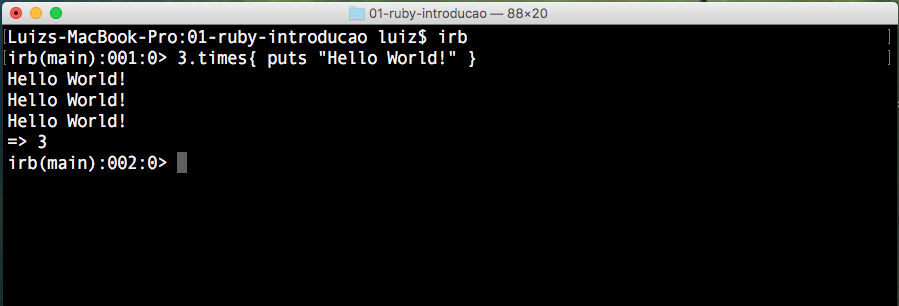
\includegraphics[scale=.35]{imagens/ruby-irb.png}
  \end{figure}
\framebreak
  \begin{itemize}
  	\item Permite a \alert{execução} de \alert{scripts} contendo vários comandos
  \end{itemize}
  \begin{figure}[hbt]
    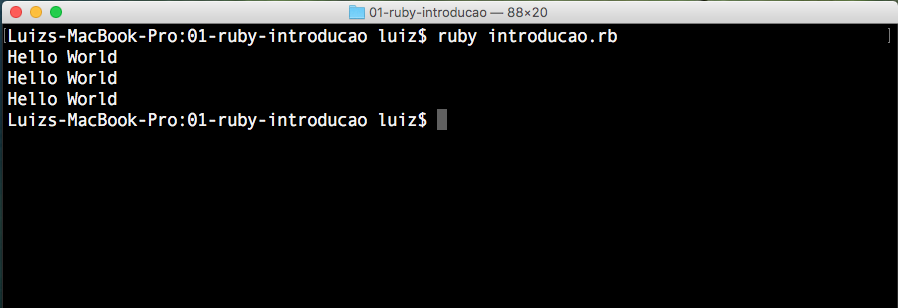
\includegraphics[scale=.35]{imagens/ruby-interpretador.png}
  \end{figure}
\end{frame}
%-------------------------------------------------------------------------------------- Início
\begin{frame}[fragile,t]{Exercícios}
  \begin{itemize}
    \item Escreva um script Ruby para imprimir um nome lido teclado 5 vezes.
  \end{itemize}
\end{frame}
